
\section{変数間関係の指標}
さて，最後のセクションは複数の変数を対象にした指標の話です。ここまでの記述統計量(平均値，中央値，最頻値，分散，標準偏差，四分位，パーセンタイル，最小値，最大値，範囲)はいずれも1つの変数に対して計算される量でした。今度は身長と体重とか，国語の点数と算数の点数といった，2つの変数がどういう関係にあるかを示す指標を考えたいのです。指標の話をする前に，可視化を考えましょう。複数の変数を図にするとき，連続的な変数であれば\textbf{散布図}を描くのが直感的にもわかりやすいでしょう。

\begin{figure}[ht]
    \centering
    \includegraphics[keepaspectratio,width=8cm]{../images/05_descriptives/Rplot04_02.png}
    \caption{散布図の例}
    \label{fig::04_09}
\end{figure}

\begin{table}[ht]
    \centering
    \caption{データの一部} 
    \begin{tabular}{rlrr}
   ID  & Name & height & weight \\ 
      \hline
    1 & 曽根　海成 & 175 &  68 \\ 
      2 & 上本　崇司 & 170 &  71 \\ 
      3 & 鈴木　誠也 & 181 &  96 \\ 
      4 & 田中　広輔 & 171 &  82 \\ 
      5 & 小窪　哲也 & 175 &  83 \\ 
      6 & 長野　久義 & 180 &  85 \\ 
       \hline
    \end{tabular}
    \label{tab::04_04}
    \end{table}

図\ref{fig::04_09}に，身長と体重のデータをプロットしたものを示しました\footnote{このデータは第\ref{m04_usingR}章で使ったものと同じ，2020年のプロ野球選手のデータセットです。}。データの一部は表\ref{tab::04_04}に示した通りです\footnote{データは全体で924人分あります。}。X軸のラベルにheight(身長)，Y軸のラベルにweight(体重)とありますように，2つの変数を同時にプロットしています。左下に目立つように1点色とサイズを変えた点を打ちましたが，これは表\ref{tab::04_04}のID=1のケース，つまり曽根選手を表しています。彼は身長が175cm，体重が68kgであり，対応するX軸，Y軸をみるとちょうどその値になっていますね。このように，各点が1つのケースに対応しているのが散布図です。

これを見ると次のことがいえそうです。すなわち，身長が高い人は，体重も大きく，背が低い人は体重も小さいが多い傾向がある，と。というのも，身長が高くて体重が軽い領域(グラフの右下)や，身長が低くて体重が重い領域(グラフの左上)に点が打たれていないので，そういう人はいない，と思えるからです。この図のように，散布図に打たれた点が右上がりの方向にあると，2つの変数の間になんらかの関係があるということが推察できますね。その関係がどのようなものであれ，このような関係にあると私たちは「何があるんだろう」と考えたり，「背が高いということは体重も重いだろうな」と予測したりできます。来年チームにやってくる新しい選手が，どんなポジションでどんな特技を持っているかはわからなくても，身長が200cmだということだけ分かれば，まあ体重が60kgってことはないよな，と予測できますものね。

さて，前期後期を通じてこの授業のポイントは「見えないものを見ようとする」でした。皆さんはここで変数間の相関を推察したわけです。関係がありそうだと予測したと言ってもいいかもしれません。直接は見えない関係をデータから見いだすには，変数間関係が重要であることがお分かりいただけますでしょうか。

図\ref{fig::04_09}に示した関係は，特に「正の相関関係」と言います。方向が同じ，つまり一方が大きければ他方も大きい，一方が小さければ他方も小さい，という関係にあるからです。逆に負の相関関係というのもあります。一方が大きければ他方は小さく，その逆も成り立つような状況がそうで，散布図でいうと点が右下がりになるような散らばりをするときです。負の相関関係でも関係は関係ですから，予測できますね。

どちらの傾向もないデータは相間がない，無相関である，といいます。散布図で書くと，各点が円のように広がる形になります。無相間であれば，関係性・規則性がないので，予測はできません。性格心理学では血液型と性格は無相関である，ということがわかっていますが，この話をすると「でも僕は血液型はA型で，多くの人に几帳面な性格だ，って言われるんですよ！」と反論する人がいます。実際に授業しているとよくある質問です。何がおかしいのかわかりますか？ 心理学者の主張は「無相関である」，です。関係がない，一般的な傾向がないということです。無関係なので，A型で几帳面な人もいるし，几帳面でない人もいます。B，O，AB型で几帳面な人もいますし，そうでない人もいるというだけなのです。無相関であれば，そこから考察することはできません。

このように，変数間関係は色々な面において重要な指標です。分散がなければ情報が取り出せない，というのと同じで，相関関係がなければ関連する情報が取り出せないのです。このことを念頭に置いた上で，変数間関係を指標化することを考えましょう。

\paragraph{共分散}二変数間関係の強さを表す指標は\keyterm{共分散}{きょうぶんさん}{covariance}といいます。先程の図\ref{fig::04_09}を例にとって考えてみましょう。身長変数を$x$，体重変数を$y$とします。ID=1の曽根選手のデータは，$x_1= 175,y_1=68$のように表します。データ全体を使って身長の平均，体重の平均を計算できますが，これをそれぞれ$\bar{x},\bar{y}$と表しましょう。共分散は次の式で表されます。
\[ s_{xy} = \frac{1}{N}\sum_{i=1}^N (x_i - \bar{x})(y_i - \bar{y})\]
これはよく見ると，分散の式に似ていると思いませんか。分散の式は次のように書くのでした。
\[ s_{x}^2 = \frac{1}{N}\sum_{i=1}^N (x_i - \bar{x})^2 \]
この二乗になっているところを展開して見ると次のようになります。
\[ s_{xx} = \frac{1}{N}\sum_{i=1}^N (x_i - \bar{x})(x_i - \bar{x}) \]
こうして$s_{xy}$と$s_{xx}$を見比べるとわかりやすいと思いますが，分散は変数$x$と$x$自身との共分散であるとも言えるわけです。

もう少し違う見方をしてみましょう。共分散は\uline{それぞれの変数についての平均偏差}の積の平均である，とも言えます。$(x_i - \bar{x})$は変数$x$について，$i$さんの値が平均からどれほどずれているかを表していて，平均より上であればプラス，下であればマイナスになります。$(y_i - \bar{y})$は同様に変数$y$についての話ですが同じ個人$i$さんについてのデータでもあります。なので，ある個人$i$が，変数$x$でも平均より上，変数$y$でも平均より上であれば，この2つを掛け合わせた$(x_i - \bar{x})(y_i - \bar{y})$はプラス$\times$プラスで，プラスの数字になります。
同様に，ある人がどちらの変数でも平均より下であれば，マイナス$\times$マイナスでプラスですから，この数字は大きくなります。
この数字が小さくなるのは，ある人が一方の変数で平均より上，他方の変数で平均より下，というときです。このとき掛け合わせた数字はマイナスになるので，総和を減らすことになります。このような数字を人数文足し合わせる($\sum_{i=1}^N$)という操作ですから，最終的にプラスであれば正の相関関係マイナスであれば負の相関関係がある，ということになるわけです。

注意すべきことは，共分散の大きさは変数の単位に依存するということです。たとえば身長と体重の共分散の場合ですと，身長の単位はcm，3桁の数字で，体重は単位がkg，2桁の数字が多いでしょうから，かけ合わせたもの平均は2〜3桁の数字になるでしょう。この時の単位はcm$\times$kgでよくわかりません。ただ，身長をmmに換算し，体重をインチに換算するといったことをすると，それに応じて共分散の大きさは変わってきます。関係が同じなのに，単位を変えただけで数字が変わってしまっては困りますね。

\paragraph{相関係数}そこで\keyterm{相関係数}{そうかんけいすう}{correlation coefficients}の出番です。相関係数\footnote{ここではピアソンの積率相関係数についてのみ説明しています。相関係数は他にも，ポリコリック相関係数，ポリシリアル相関係数，テトラコリック相関係数など，色々なバージョンがあります。}は，単位に影響されずに変数間関係をみるものです。共分散の大きさは，元データの単位に依存するので，変数間関係を表す指標の大きさが単位に依存するということは，異なる変数間関係を比較できないことになって不便だからです。「身長と体重の関係の強さ」と「国語の成績と算数の成績の関係の強さ」はどっちが強い結びつきをしているのでしょう？ との問いには共分散を見ても答えられません。さてでは，それぞれの変数の単位を揃えるにはどうしたらよいのでしょう？ 

そう，標準化ですね。それぞれのデータをzスコアに計算しなおせばよいのです。変数$x$をzスコアにしたものを$z_x$と表すとして，これの共分散を考えましょう。変数$x$と$y$の相関係数は$r_{xy}$と表します。
\begin{align*}
    r_{xy} &=  \frac{1}{N}\sum_{i=1}^N (z_{x_i} - \bar{zx})(z_{y_i} - \bar{zy}) & \mbox{zスコアの平均は$0$}\\
      &= \frac{1}{N}\sum_{i=1}^N z_{x_i} z_{y_i}  & \mbox{zスコアの式に戻そう}\\
      &= \frac{1}{N}\sum_{i=1}^N \frac{(x_i - \bar{x})}{s_x} \frac{(y_i -\bar{y})}{s_y}  & \mbox{$i$は分子にしか関係ないから}\\
      &= \frac{\frac{1}{N}\sum_{i=1}^N (x_i - \bar{x})(y_i -\bar{y})}{s_xs_y}  & \mbox{分子が共分散だ}\\
      &= \frac{s_{xy}}{s_xs_y}  & \\
\end{align*}

このように展開できました。相関係数は共分散をそれぞれの標準偏差で割ったもの，と考えれば良いわけですね。この数字は単位が違う2つの変数でも計算できますし，単位が整えられているので$-1 \le r_{xy} \le 1$の範囲に収まります。

\begin{figure}[ht]
    \centering
    \includegraphics[keepaspectratio,width=8cm]{../images/05_descriptives/Rplot04_03.png}
    \caption{様々な相関係数}
    \label{fig::04_10}
\end{figure}

図\ref{fig::04_10}には様々な相関係数のプロットを示しました。ちなみに先程の野球選手の身長と体重のデータは，相関係数$r=0.601$になります。大体の散布図のイメージを持っておいてもらうことも重要ですし，何かデータを取ったら図にする，ということを忘れないでください。


\subsection{相関係数の落とし穴}
最後に，相関係数を見る時の注意を5つあげておきます。いずれも数字だけ見るのではなく，データの散布図やその意味をしっかり考えれば引っ掛かりはしないのですが，実際のデータ分析をするときは(あまりにも簡単に相関係数が計算できてしまうがために)，見落とされることが多いケースでもあります。よく読んで注意するようにしておいてください。

\paragraph{落とし穴1；直線じゃないかも}
図\ref{fig::04_10}の左上には$r=-1$の例，右下には$r=+1$の例があります。このように，相関係数はその極限で，直線になる関係であることを理解しておいてください。言い換えると，相関係数はあくまでも変数間の直線的関係を指標化したものであって，曲線的な関係の場合はうまく表現できないのです。図\ref{fig::04_11}には曲がった散布図の例を示しました。このデータの相関係数は$r=0.005$です。ほとんど関係ないですね！じゃあこのX軸の変数とY軸の変数は何の関係もない，といっていいでしょうか。例えばこのデータ，X軸がコーヒーの温度，Y軸が美味しさだったらどうでしょう。熱すぎても冷たすぎても，コーヒーは美味しくありません。適温というのがあるのです。あるいはX軸が血圧，Y軸が健康度だったらどうでしょう。血圧も高ければ高いほど健康，低ければ低いほど不健康というわけではないですよね。これらの例にあるように，心理的なデータや整理的なデータというのは，中庸であることが重要であることがあります。その時に相関係数を算出して，それがとても低いので「血圧と健康には関係がない」と結論づけるのは間違えています。直線性を表す指標がよくない，というだけなのですから。

\begin{figure}[ht]
    \centering
    \includegraphics[keepaspectratio,width=8cm]{../images/05_descriptives/Rplot04_04.png}
    \caption{曲がった関係には向かない}
    \label{fig::04_11}
\end{figure}

\paragraph{落とし穴2；全体の傾向じゃないかも}
逆に，ある2変数の相関係数が$r=0.922$でした。この2変数には強い相関があるといって良いでしょうか。待って待って，一旦落ち着いて散布図を書いてみましょう。例えば図\ref{fig::04_12}のようなデータなのかもしれないのですから。
\begin{figure}[ht]
    \centering
    \includegraphics[keepaspectratio,width=8cm]{../images/05_descriptives/Rplot04_05.png}
    \caption{外れ値がひっぱる}
    \label{fig::04_12}
\end{figure}
図\ref{fig::04_12}は，確かに相関係数は高いのですが，明らかにおかしなポジションにいるデータが1件ありますよね。平均値が外れ値に引っ張られたように，平均値をその計算新規の中に取り込んでいる相関係数も，外れ値に弱いところがあります。今回この極端な値を取る1ケースを取り除くと，相関係数は$r=0.3$にまで下がります。左の小さな群だけで見れば，むしろ関係ないと考えるべきなのです。これもデータを図にしなければ気づかない落とし穴です。

\paragraph{落とし穴3；データの一部が切り取られている? }
とある大学の入学試験のデータを取ってみたとします。入試の成績と，入学後の成績のデータを集め，入試の成績がどれぐらい入学後の成績と関係があるのかを考えたい，というわけです。良い成績で入学したら，入学後も成績が高いというのが普通に考えられる結果ですが，実はその相関係数は$r=0.4$ぐらいだった，ということもあります。なぁんだ，入試の成績はその後の頑張りと関係ないんじゃないか，入試なんか意味がないんじゃないか，と思うのは大間違い。

さて図\ref{fig::04_13}には，X軸に入試の成績を，Y軸には入学後の成績をプロットしてみました。相関係数は全体で0.7あるのです。ところが，大学入試というのは世知辛いもので，ある点数を取らない人はそもそもその大学に入れませんよね。図でいうと，ある線(60点)より右側の黒いデータしか分析する時に手に入らないのです。この黒い点だけみて相関係数が低いから，関係ないんだと思ってしまうのは間違いです。このように，データがそもそも打ち切られている可能性にも注意が必要です。このようなデータは切断データといわれます。これは相関係数の問題というより，データの問題なのですが，データの性質をよく考えて考察しなければならないということはしっかり意識しておいていただきたいところです。

\begin{figure}[ht]
    \centering
    \includegraphics[keepaspectratio,width=8cm]{../images/05_descriptives/Rplot04_06.png}
    \caption{打ち切りデータの例}
    \label{fig::04_13}
\end{figure}

\paragraph{落とし穴4；データは色々な情報が混在している? }
図\ref{fig::04_14}の左を見てください。これは右上がりの散布図ですから，なるほど変数間に関係はありそうです。実際に相関係数を計算すると$r=0.67$になります。今度は散布図もみているからバッチリ！と思うかもしれませんが，さにあらず。
実はこのデータ，3つのグループのデータが混ざった全体的な傾向です。図の左側には，グループごとに色分けをしてみました。おや，これを見るとグループの中ではむしろ右下がりの分布をしていませんか？ 実はその通りで，グループAは$r_A=-0.29$，グループBは$r_B=-0.42$，グループCは$r_C=-0.35$と，いずれも負の相関をしているのです。にもかかわらず，全体で見ると正の相関をしている，ということもあるわけですね。

\begin{figure}[ht]
    \centering
    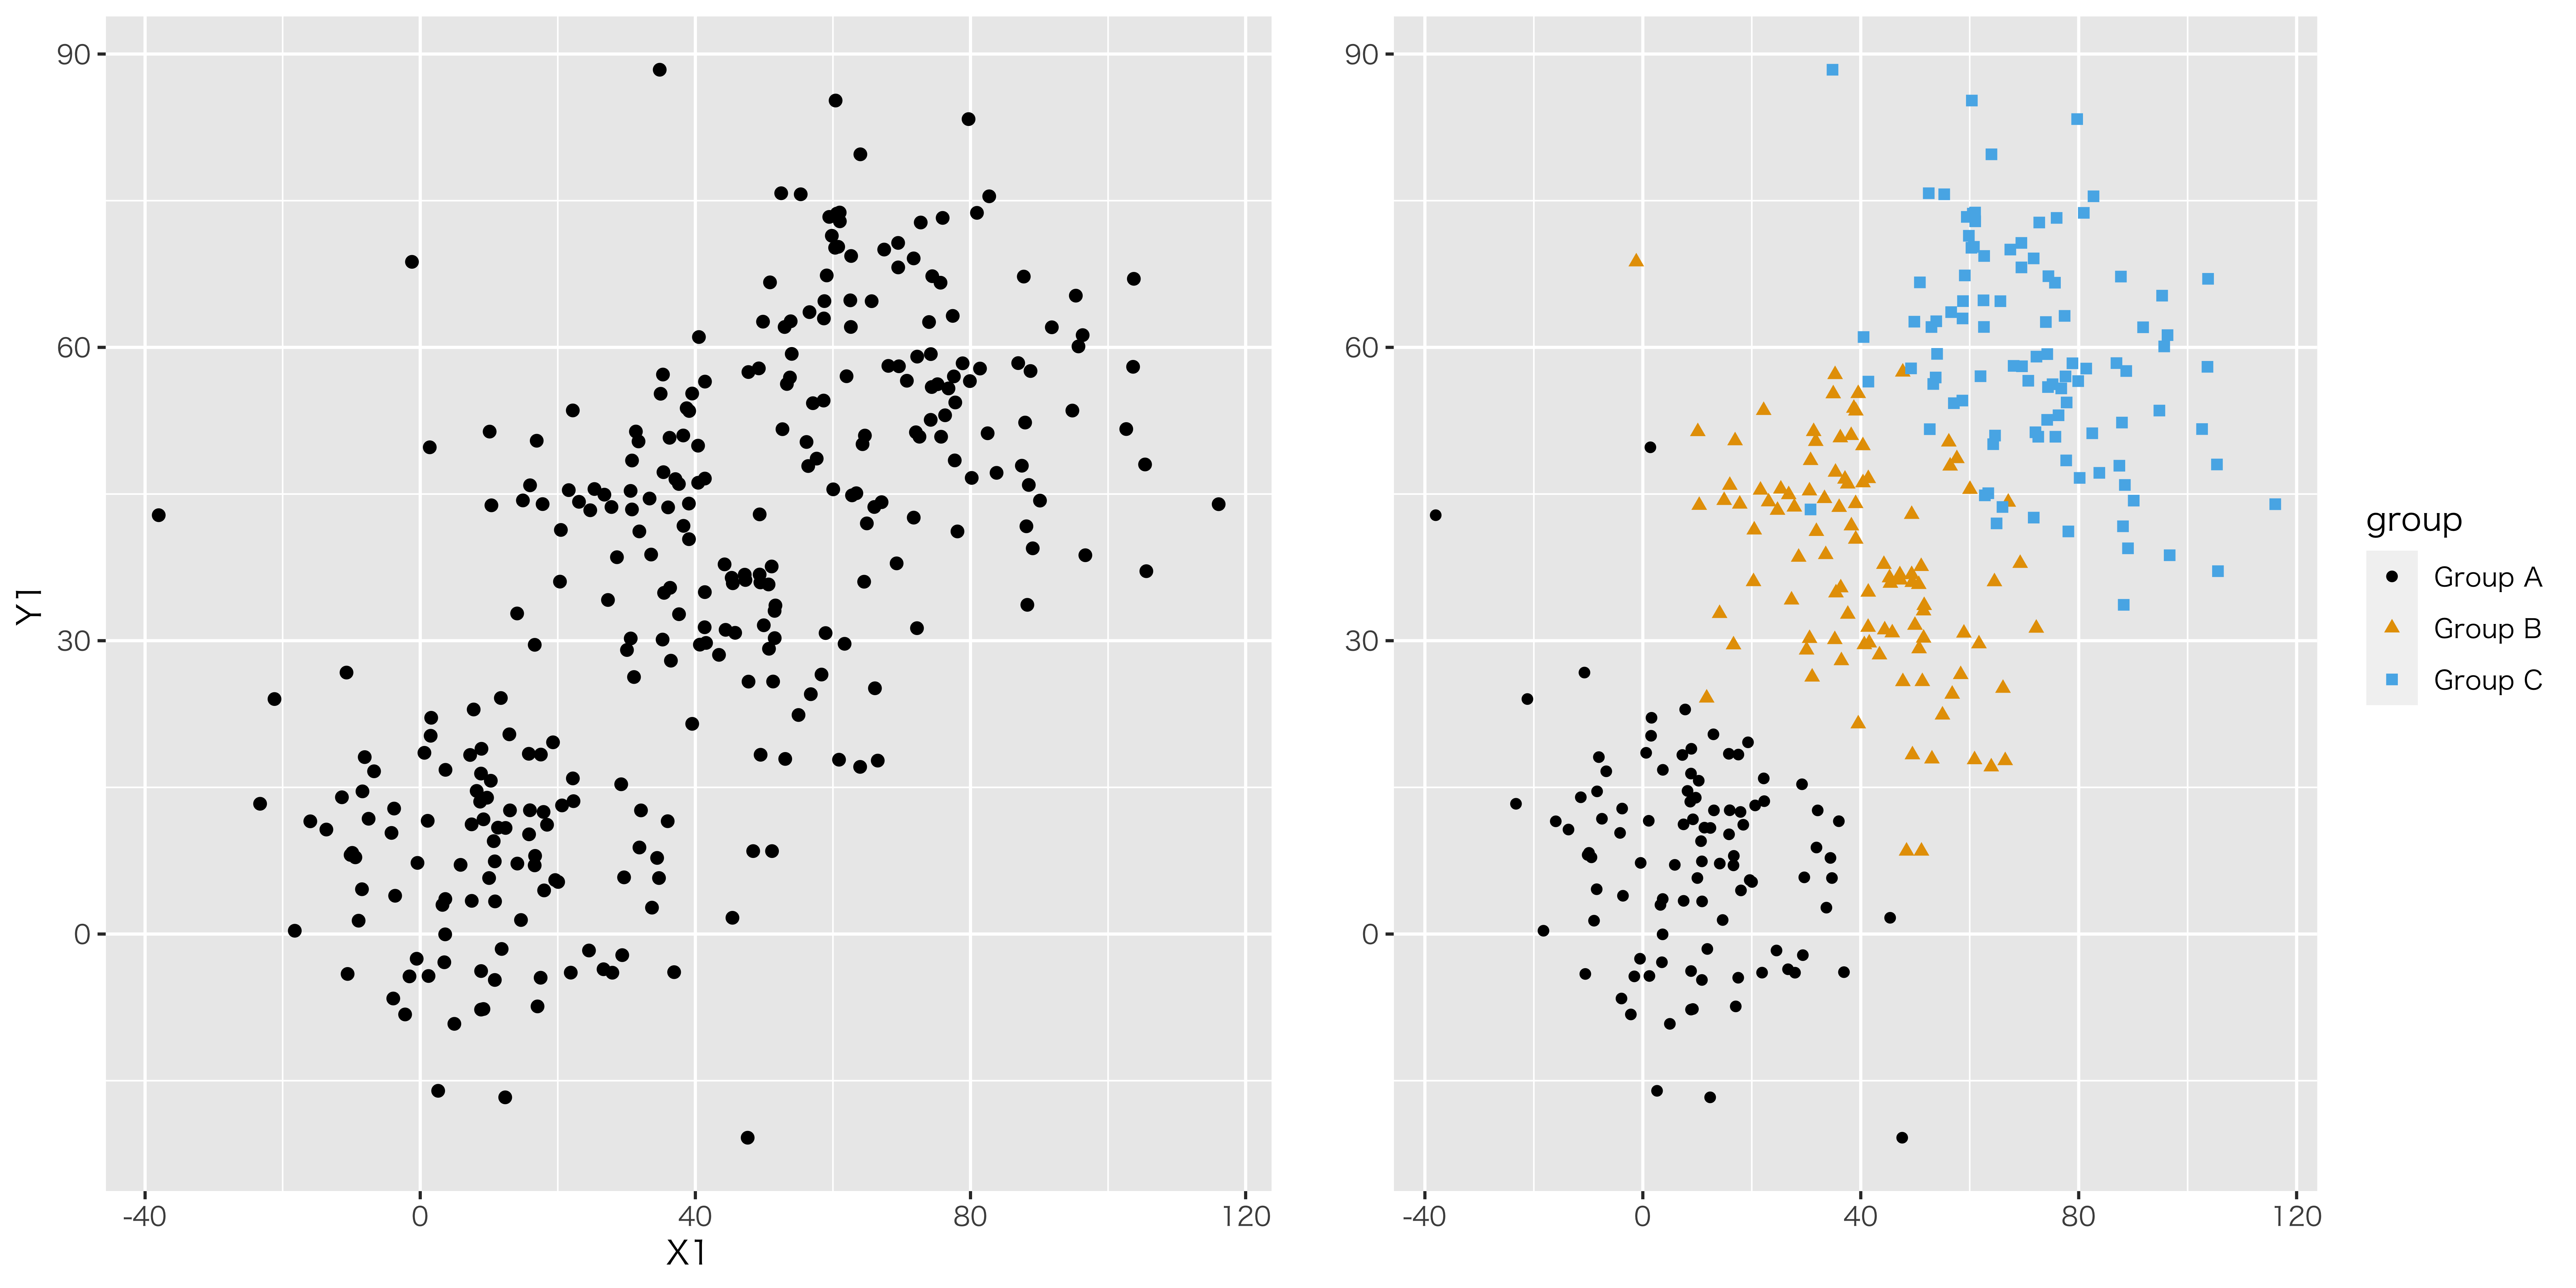
\includegraphics[keepaspectratio,width=8cm]{../images/05_descriptives/Rplot04_07.png}
    \caption{階層的なデータ}
    \label{fig::04_14}
\end{figure}

このデータ，例えばX軸がゲームで遊ぶ時間，Y軸が学校の成績だったとしますと，全体で見るとゲームをすれば成績が上がる，という結論になってしまいますね。でも学校別(グループ別)でみるとむしろ逆，ここにあるのは3つの学校のそもそもの成績の違いが反映されているだけでした，ということもあるわけです。このように，外的な指標で群が変わることがわかっているなら，プロットする時にその情報を加えて，このような情報の混在が生じていないかをチェックする必要があります。プロットするのは当然ですが，プロットのやり方にも注意が必要なのですね。また，群ごとの違いがわかっていなくても，潜在的に何か違うグループに分かれているのかもしれません。回答者の特性を考慮して，いくつかのクラスターに分けて分析するという手法も統計的に考えられています。データを色々な角度から見る，という姿勢は忘れてはいけません\footnote{マーケティングの領域では，セグメンテーションと呼ばれることもあります。購買層ですね。クラスターというのはCOVID-19の関係で一般的な用語になりましたが，この言葉そのものに悪い意味はなく，塊という意味です。}。

\paragraph{落とし穴5；相関と因果を取り違えてはいけない}
他にも例えば次の変数間には高い相関があることがわかっています\footnote{参考；\url{http://tylervigen.com/spurious-correlations}}。
\begin{itemize}
\item ニコラス・ケイジ映画出演数とプール溺死数
\item マーガリン消費率とメイン州の離婚率
\item 自分のベッドシーツに絡まって死んだ人の数とチーズ消費量
\end{itemize}

このように，相関があるからと言って意味があるわけではありません。おそらくニコラス・ケイジ(ハリウッド俳優)が頑張って映画に出たからといって，米国でのプール溺死者数が増えるわけではないし，マーガリンを塗らなければ離婚率が下がるというものでもないでしょう。ただデータを取ると，見かけ上，相関係数が高くなってしまっただけなのです。こうした関係のことを\textbf{疑似相関}と言います。我々は目に見えない心理学的な現象を，相関関係を手掛かりに分析していくのですが，たまたまみられる表面的な関係性を「ほらやっぱり！」と思い込んでしまわないように，慎重に考えなければなりません。

また，相関関係はどちらかが原因でどちらかが結果であるという，因果関係を示すものでもありません。先の例でいうと，マーガリンを塗るから離婚する，という関係があるわけではないのです。ほかにも町の消防署の数と火事の件数にも相関関係があります。これは消防署の人間が町に火をつけて回ってるわけではないですよね(むしろ逆)，相関関係を因果関係と取り違えると大変なことになりますので，この点にも注意が必要です。

相関係数という関係を探るヒントは強力ですが，時にミスリーディングにもなります。これらの注意点にも常に配慮しつつ，目に見えない本当の関係を見つけ出さなければなりません。厳しいですねえ。



\subsection{推論}
主観確率のように，自分の考えていることを確率で表現することの例を考えてみましょう\footnote{このサブセクションのお話は，\citet{Maeda2017}の2章の受け売りです。この本はとてもいい本ですから，ぜひ読んでみてください。私も監訳者の1人ですから，宣伝です!}。

ある日，朝起きたら家の前の地面が濡れていたとします。何があったのか，と考えますよね。昨日寝ている間に雨が降った？ 散水車が通った？ 水道管が破裂した？ 通行人が飲み物をこぼした？ 他にもいろんなパターンが考えられるかもしれませんが，とりあえずこの4つの可能性を考えたとしましょう。これで考えられる可能性は全部だ，とします。そこでさっき考えた「可能性」を検証していくことにします。
\begin{enumerate}
    \item 気象庁に電話して，昨晩雨が降ったか確認した→降ってなかったとします。
    \item 市役所に電話して，昨晩散水車が通ったか確認した→通ってなかったとします。
    \item 水道局に電話して，昨晩水道のトラブルがあったか確認した→特にそういった問題はなかった，とします。
\end{enumerate}
このように考えていくと，残る最後の可能性，「通行人が飲み物をこぼしたに違いない」と我々は結論づけるしかありません。かのシャーロック・ホームズも次のように言っていたではないですか。

\begin{quote}
    なんども言っているだろう？ ありえないことを全て取り除いて，それでもなお何かが残るのであれば，それが真実に違いないさ。たとえどんなに可能性が低そうに見えてもね。
\end{quote}

ここで示したように，我々が推論するというのは実は，確率の言葉で表現できるのです。図\ref{fig::07_01}には，朝起きて初めて地面が濡れているのをみた時の状況を表しています。考えうる可能性は4つあって，どれが正しいのかわからない状態です。どれが正しいのかわからないというのはつまり，有力な手がかりがないわけですから，どれも同じぐらい怪しいというか，どれも同じぐらいしか確信が持てないでいます。可能性は4つあって，全体が1.0でなければならないとすると，各事象(推理)に与えられる確率は25\%ずつということになります。

\begin{figure}[ht]
    \centering
	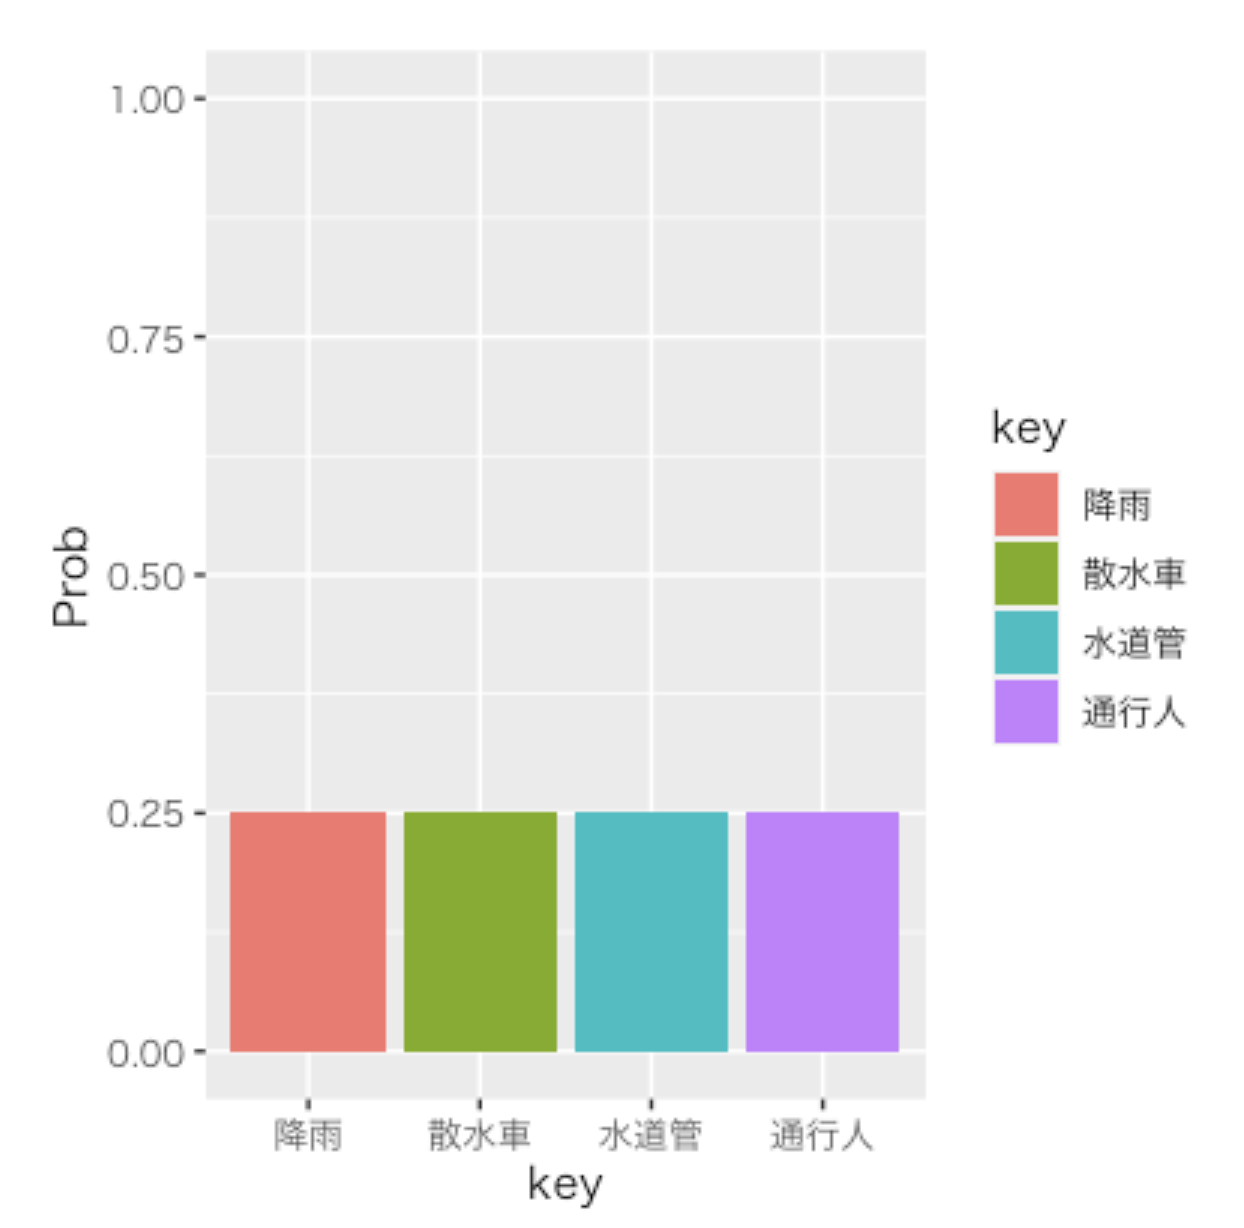
\includegraphics[keepaspectratio,width=8cm]{../images/07_probability/slide07_01.png}
    \caption{最初の状態。有力な手がかりはない。}
    \label{fig::07_01}
\end{figure}

ここで気象庁に電話をしたとしましょう。すると雨は降っていなかった，という情報が手に入ったわけです。これを受けて，「雨が降った可能性は0だ」と考えることができます。確率で表現するためには全部の確率(可能性)の和が1.0でなければなりませんから，残りの3つの確率＝確信度が33\%に上がったことになります(図\ref{fig::07_02})。
\begin{figure}[ht]
    \centering
	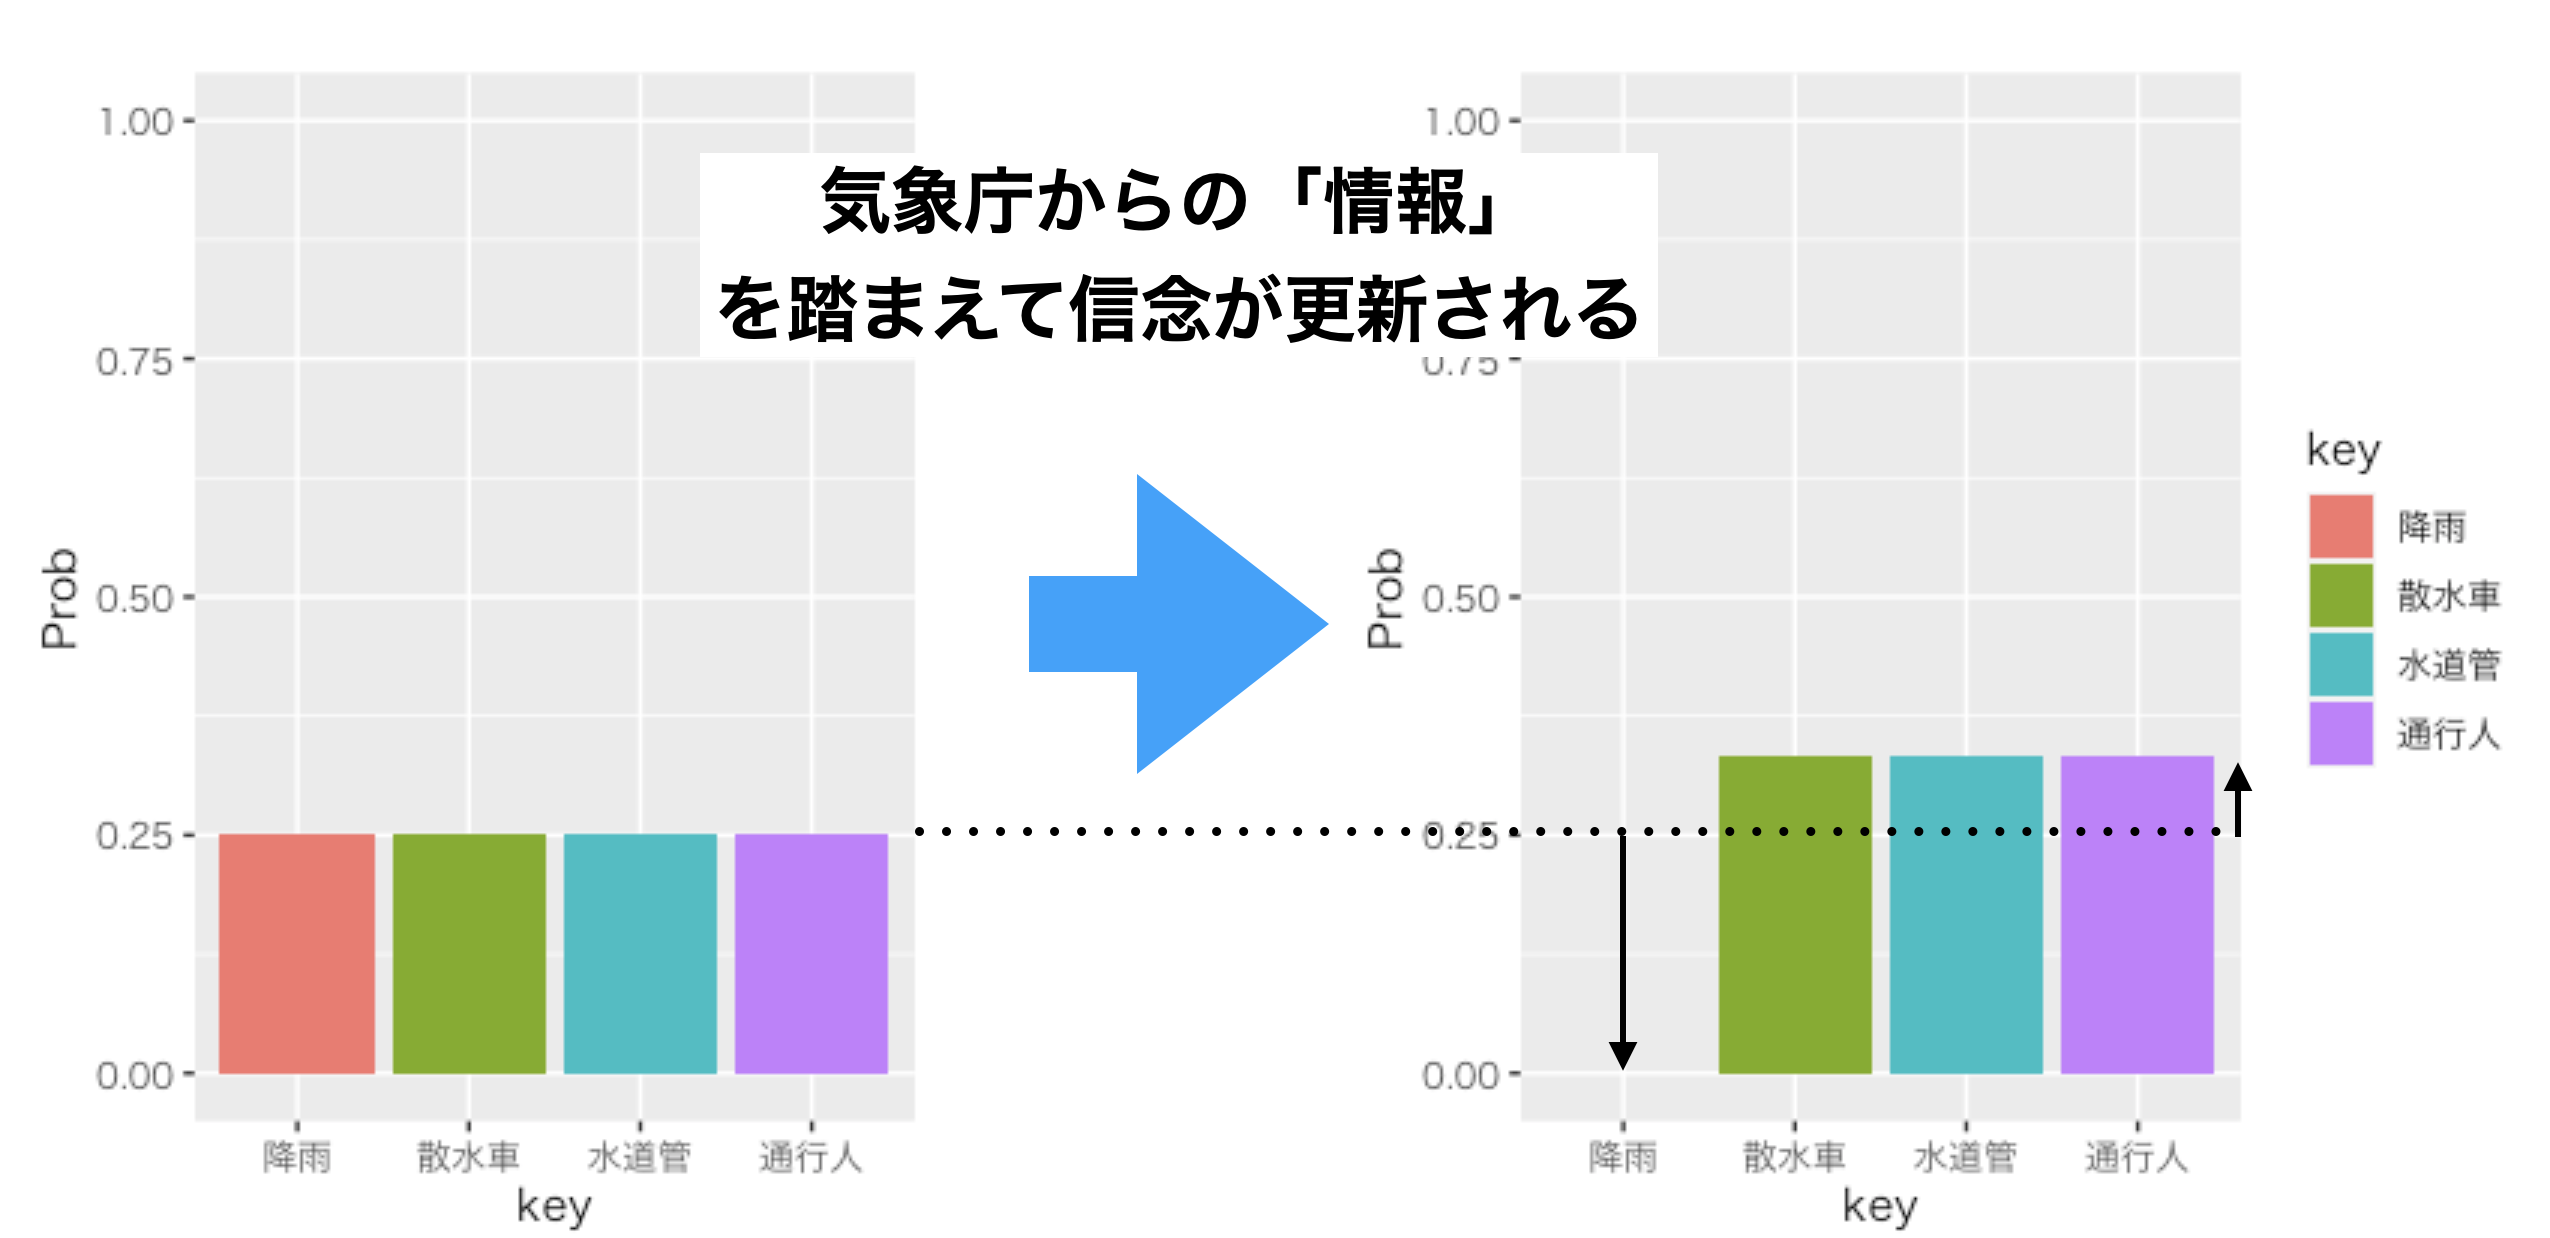
\includegraphics[keepaspectratio,width=8cm]{../images/07_probability/slide07_02.png}
    \caption{雨が降ったという可能性はゼロになったので，確信度がかわった。}
    \label{fig::07_02}
\end{figure}

次に同じように，今度は市役所に電話して，散水車の可能性を確かめました。そうするとそんなことはしていない，という情報が手に入ります。これを受けて「散水車が通った可能性も0だ」と考えが変わります。確率で表現するなら，選択肢が2つに減りましたがどちらも同じぐらいの確からしさしかないので，50\%ずつに確信度が変わった，ということです(図\ref{fig::07_03})。
\begin{figure}[ht]
    \centering
	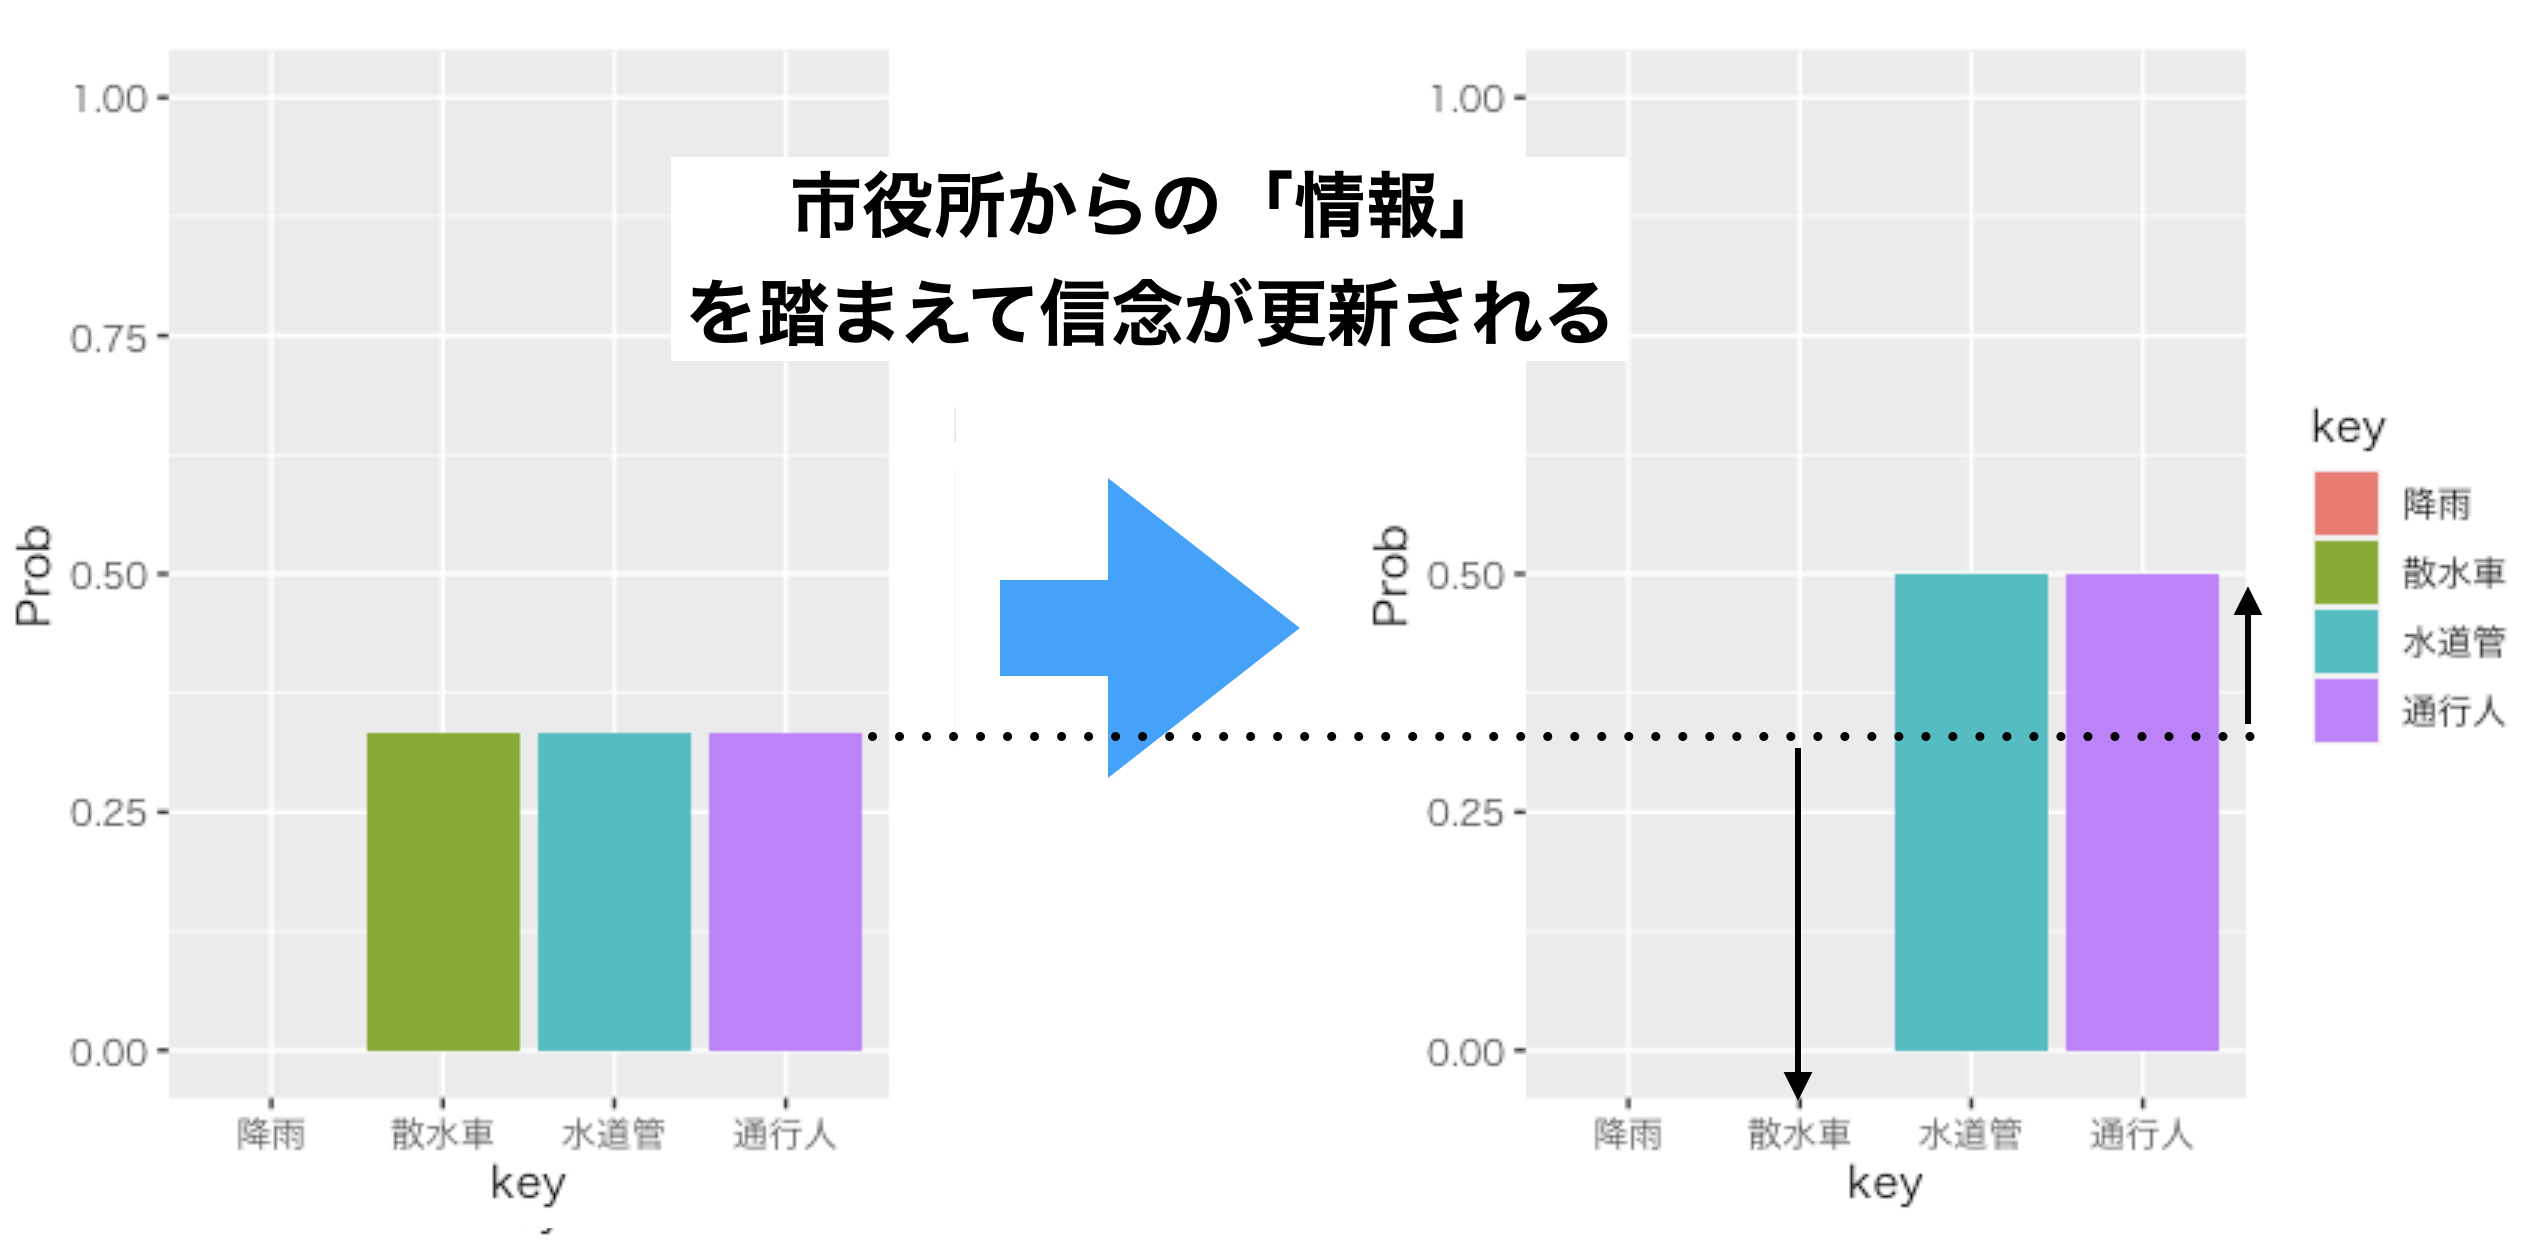
\includegraphics[keepaspectratio,width=8cm]{../images/07_probability/slide07_03.png}
    \caption{散水車が通った可能性はゼロになったので，確信度がかわった。}
    \label{fig::07_03}
\end{figure}

最後に水道局に確認して，水道の問題でもないことがわかりました。これを受けて，シャーロック・ホームズばりに「あり得ないことかもしれないが，通行人が飲み物をこぼしたとしか考えられない」という状態になるわけです。確率でいうなら，他の事象の可能性がゼロで，全部の面積が1なのですから，100\%間違いない！ということです。
\begin{figure}[ht]
    \centering
	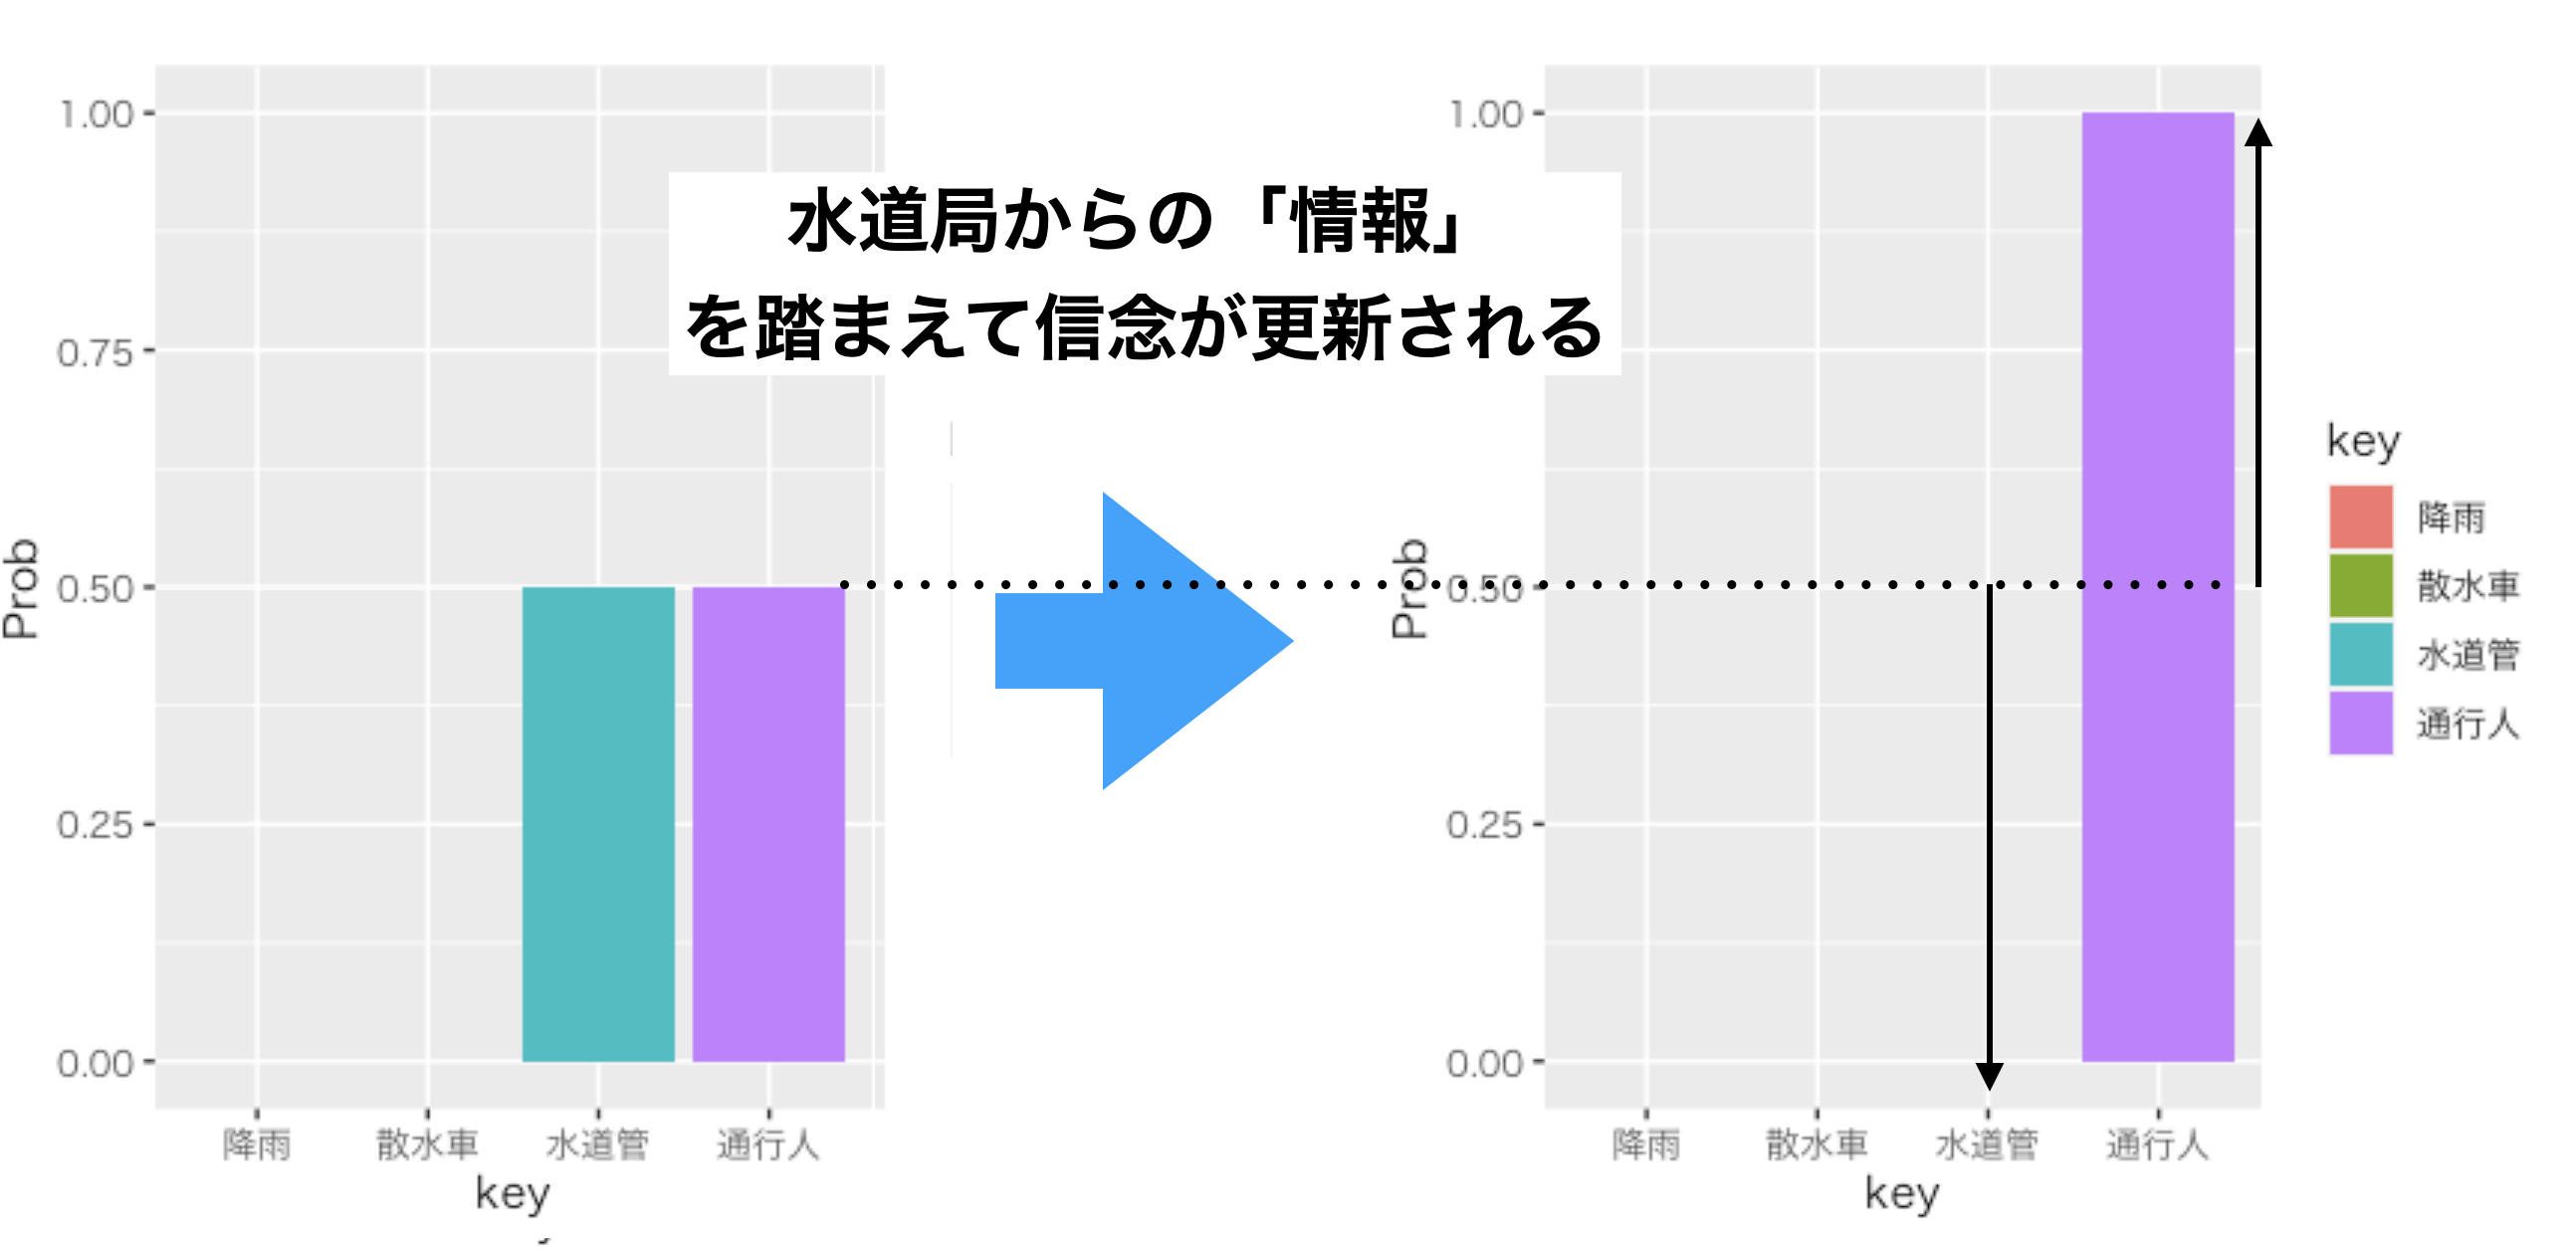
\includegraphics[keepaspectratio,width=8cm]{../images/07_probability/slide07_04.png}
    \caption{水道管が破裂した可能性はゼロになったので，確信度がかわった。}
    \label{fig::07_04}
\end{figure}

このように，確率は確信度を表現する数字として使うことができます。またこのお話にあったように，我々は「情報を得て，推論する」のです。情報を得ることで確率が変わるのがポイントで，心理学者がデータをとって分析するのも，データという情報があることで考えが前に進むからです。また\textbf{推論とは確率を再分配すること}とも言えます。より確からしいものに考えを進めていく，科学という営みはデータで確信度をアップデートする＝確率の値を再分配していくことだとも言えます。


\section{確率関数の期待値}
\label{expectation}
最後に確率分布関数の特徴を記述することについて触れておきます。
確率分布とは，確率的に変動する数字の実現値と，出現確率を一覧にしたもので，確率質量関数や確率密度関数で表現されるのでした。
離散変数であれ，連続変数であれ，いろいろな数字が出てくる可能性があるので，その特徴を記述する方法をみておきましょう。
ここでは確率分布の平均と分散を考えます。確率分布の平均は特に\keyterm{期待値}{きたいち}{expectation}と呼ばれます。

確率的にしか得られない数字に対して，平均的にどれぐらいの数字が得られるか，は「トータルどの程度の数字が期待できるか」という意味で期待値と呼ぶのです。
サイコロの例で説明しましょう。サイコロの出目は1，2，3，4，5，6ですが，サイコロを振って出る目の平均はどれぐらいの値になるのか？ を考えます。ここではもちろん正当なサイコロ，出目がいずれも$1/6$の確率であることとします。
確率変数$X$の期待値は$E(X)$で表し，次のように計算します。

\[ E(X) = \sum x_i \times p_i \]

ここで$x_i$は確率変数がとりうる値，$p_i$はその値が出てくる確率です。そしてすべての可能性を足し合わせ($\sum$)ます。
サイコロの期待値は次の通りです。
\[1\times\frac{1}{6}+
2\times\frac{1}{6}+
3\times\frac{1}{6}+
4\times\frac{1}{6}+
5\times\frac{1}{6}+
6\times\frac{1}{6}
=3.5\]
実際に3.5という出目があるわけではありませんが，平均はこうなるということです。このように，確率分布の平均値は実現値$\times$その確率を全て足し合わせたもの，と思っておいてください。
例えば，これがわかれば宝くじの期待値がわかります。2004年のサマージャンボ宝くじ，1ユニット，1000万通り当たりの当選金は表\ref{takarakuji}のようになります。


\begin{table}[hb]
    \centering
    \caption{2004年のサマージャンボ宝くじ当選金一覧}
    \begin{tabular}{cccc}
等級 & 当選金 & 本数 & 当選確率 \\\hline
1等 & 2億円 & 1 & 0.00001\% \\
前後賞 & 5千万円 & 2 & 0.00002\% \\
組違い & 10万円 & 99 & 0.00099\% \\
2等 & 1億円 & 1 & 0.00001\% \\
3等 & 100万円 & 10 & 0.0001\% \\
4等 & 10万円 & 100 & 0.001\% \\
5等 & 3000円 & 100000 & 1\% \\
6等 & 300円 & 1000000 & 10\% \\
夏ラッキー賞 & ラッキー賞 & 40000 & 0.4\% \\
    \end{tabular}
    \label{takarakuji}
\end{table}
これを元に期待値を計算すると次のようになります。

\[200000000 \times 0.0000001 + 50000000 \times 0.0000002 + \cdots + 10000\times0.4=143.0 \]

宝くじは一枚300円で買えますから，300円買っても平均143円しか当たらないことになります。言い換えると157円=$52\%$は胴元の儲けになるので，ギャンブルとしては効率が悪い部類に入ることがよく知られています\footnote{外国では，「宝くじは貧乏人の税金だ」などと言われることもあるようです。一攫千金を求めてつい・・・ね。}\footnote{ちなみにこれは「バラ」で買った場合です。連番で買うとちょっと計算がややこしいです。}。

話を戻します。このようにして，(離散)確率分布関数の平均値が計算できます。平均値だけでなく，分散も計算できます。式は次のようになります。

\[ Var(X) = \sum (x_i-E(X))^2 \times p_i \]

実際の出目から期待値を引いたものの二乗に，その確率をかけたものを総和するのですね。サイコロの場合は次のようになります。

\[
    (1-3.5)^2\frac{1}{6}+
(2-3.5)^2\frac{1}{6}+
\cdots+
(5-3.5)^2\frac{1}{6}+
(6-3.5)^2\frac{1}{6} = 2.9166...
\]

連続分布の場合は足し算でなく積分をすることになりますが，基本的な発想は同じです。

以上，今回は確率の基本的なお話でした。



\section{標準正規分布の面積を測る}
\label{MeasureTheNDarea}
さて，正規分布の確率密度関数の形がわかりました。これは連続分布ですから，縦軸は\keytermL{確率密度}{かくりつみつど}であることに注意してください。
また定義上，「ある点の確率」は存在しません。確率は，幅を持った面積で表されることも思い出してください($\to$ Pp.\pageref{continuousDistribution})。

例えば標準正規分布において，確率点$0.3$から$1.0$までの面積(確率)を求めたいとします。図\ref{fig::08_08}の範囲ですね。
これをどのようにして求めるのか，4つの方法をご紹介しましょう。
\begin{figure}[ht]
    \centering
	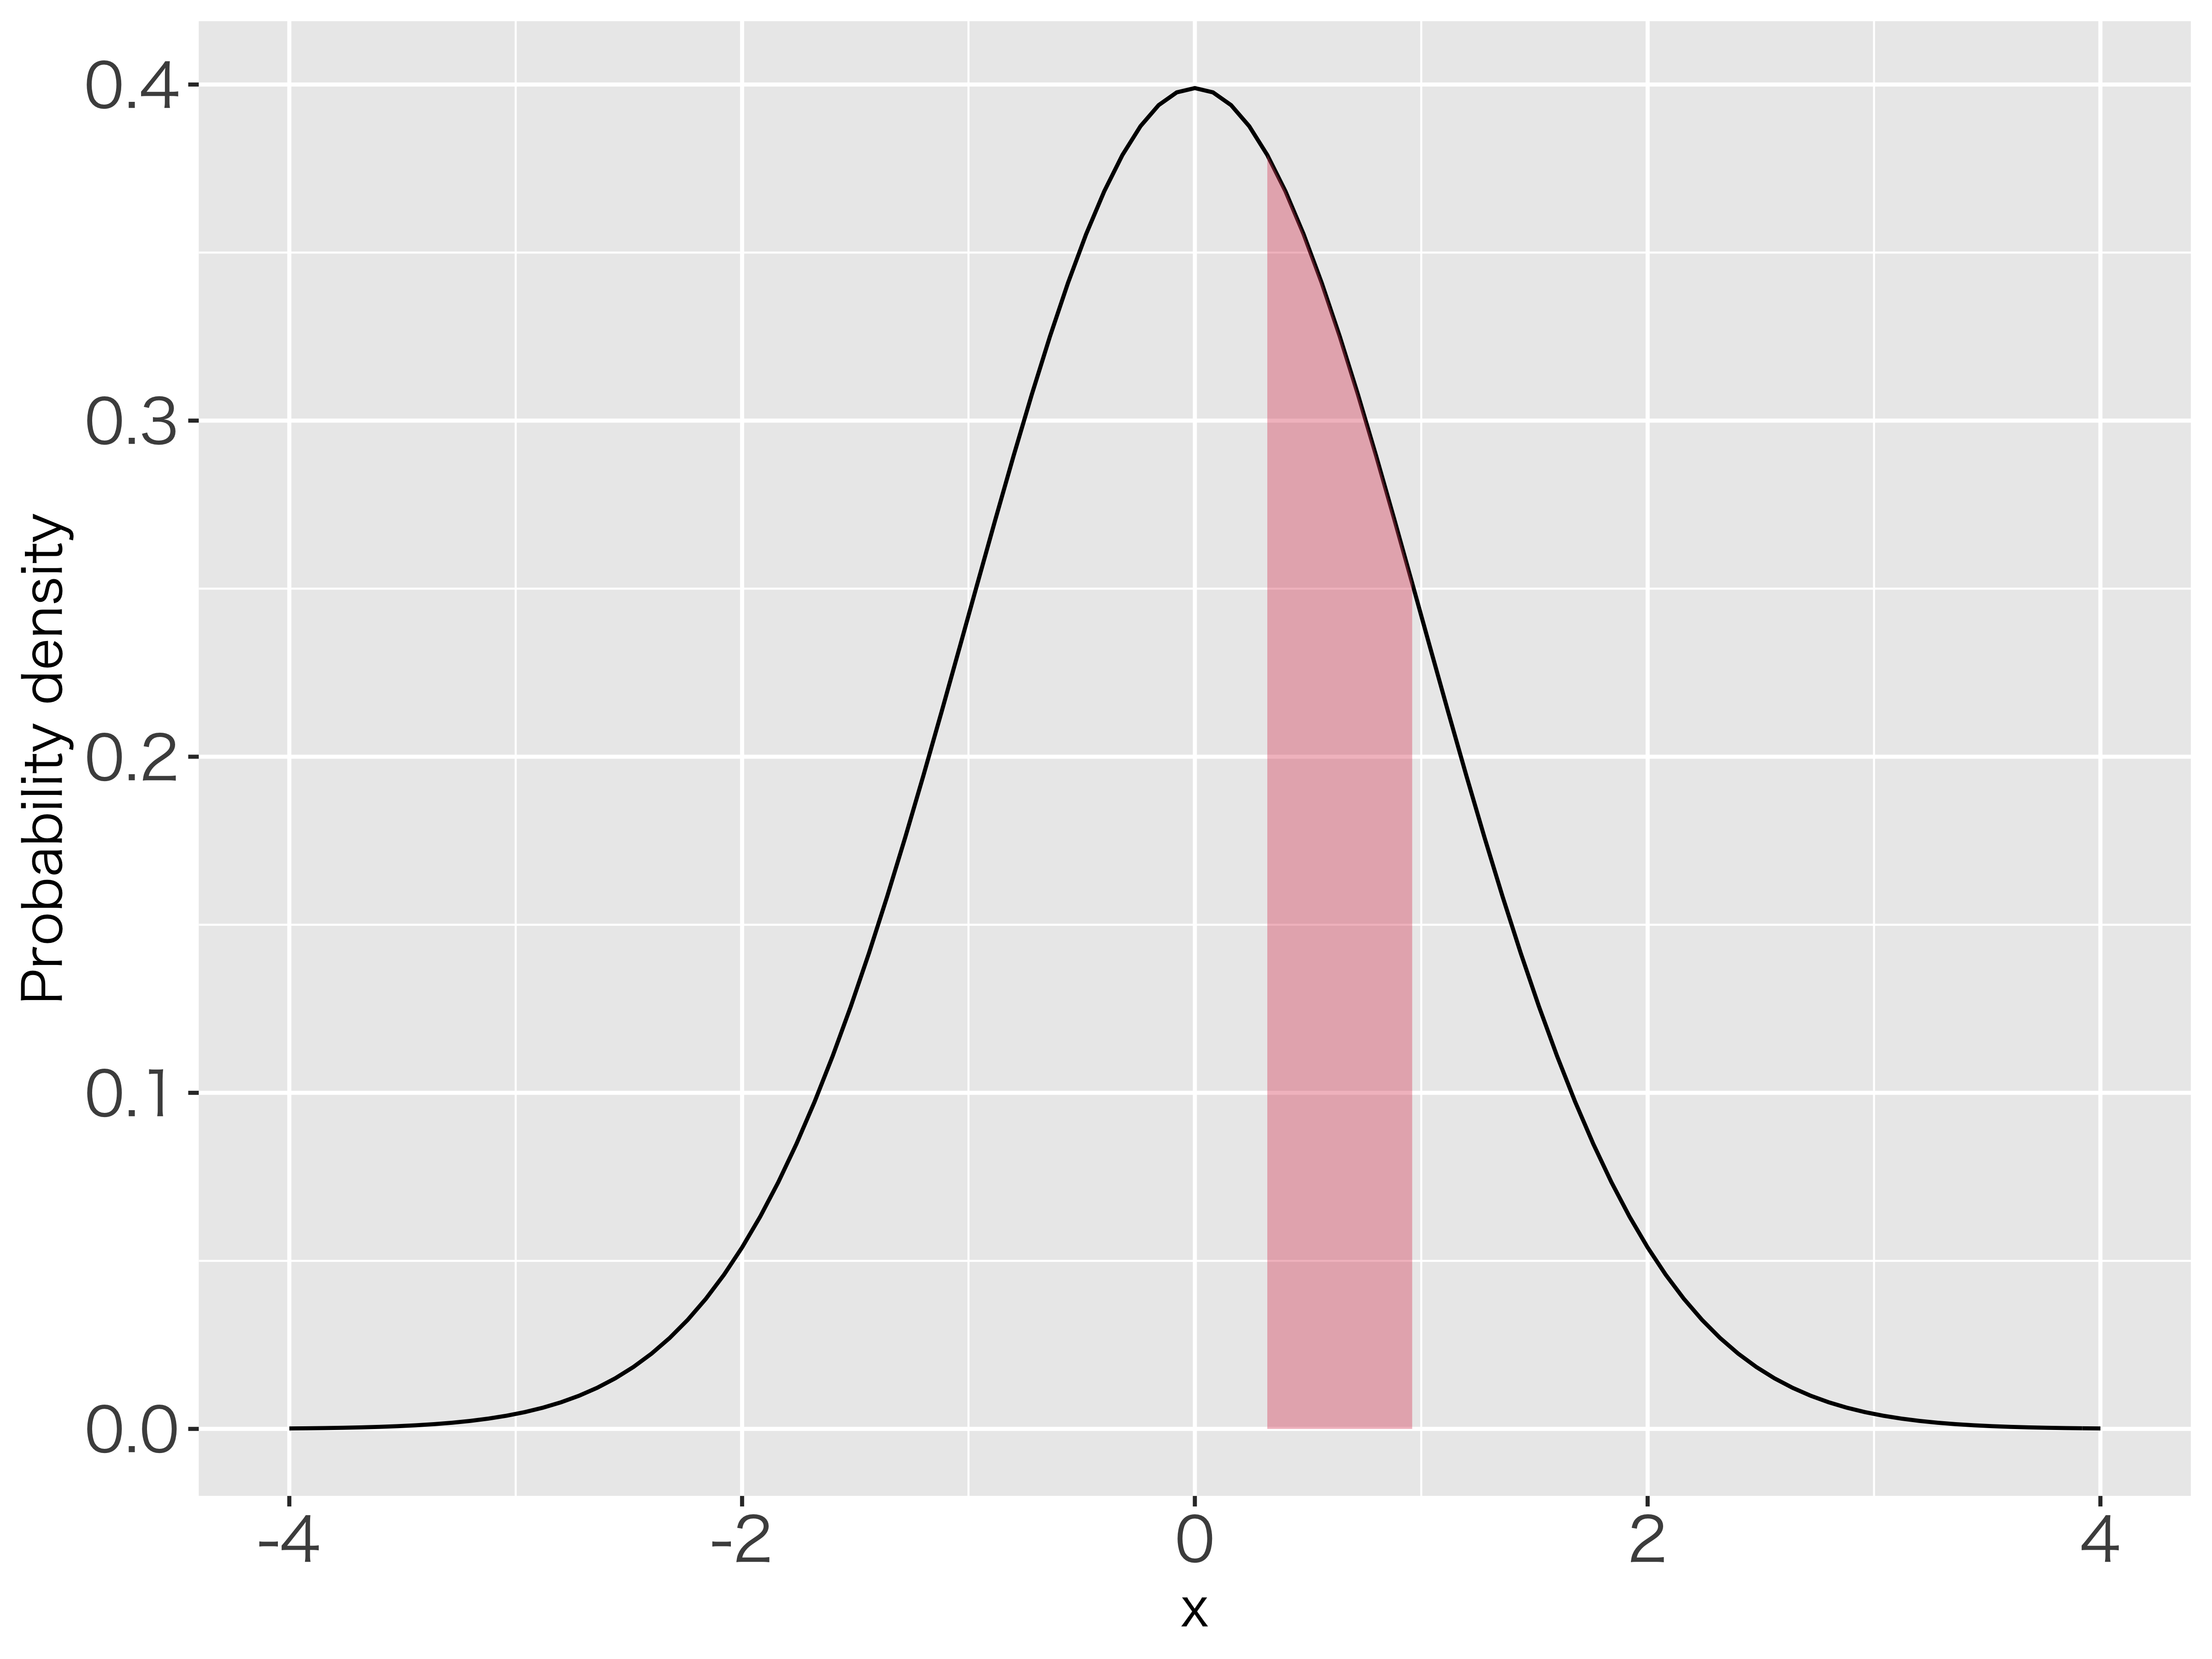
\includegraphics[keepaspectratio,width=8cm]{../images/08_CorrelationCausation/Rplot08_03.png}
    \caption{正規分布の確率を求める}
    \label{fig::08_08}
\end{figure}

\paragraph{計算する} 正しく算出するためにはもちろん，関数の形から計算すれば良いのです。当たり前と言えば当たり前ですが，計算式は次のようになります。
\[ p(x) = \int_{0.3}^{1.0} \frac{1}{\sqrt{2\pi}} exp(-\frac{x^2}{2}) =0.2234333...\]
このように面積を求めるのは積分になります。$\int$というのは積分記号で，$0.3$から$1.0$の範囲の面積を求めよ，としてその右に関数を書きます。この計算ができるのであれば何より正確で，22.34\%
なんだな，ということがわかります。

しかし積分の計算に慣れていない人にとっては難しいですね\footnote{特に文系には！私も文系出身ですので，最初に習った頃は「うん，わからん！」となりました。}。そこで次の方法をご紹介します。

\paragraph{数表を見る} 2つ目の方法は数表を見る，です。数表とは数字の表のこと。何を言ってるんだと思うかもしれませんが，心理統計のテキストにはたいてい付録として数表がついているものでした。代表的な関数については，ある程度計算したものの一覧表があると，計算機を使う必要がないから便利だったのですね。あるいはそうした表だけがのっている数表の本というのもかつてはありました\footnote{過去形で書いていることからも明らかなように，これら数表が便利だったのは現在ほどコンピュータが個人消費者レベルにまで浸透していない時代のことで，今は次に紹介する計算機を使う方が素早く正確です。}。数表の例を\ref{tbl::08_01}に挙げます。


\paragraph{計算機を使う} さてさて，数表を見るのは大変面倒だということがわかりました。これなら積分計算をした方が早いくらいかもしれません。実用的にはもちろんこんな面倒なことはしません\footnote{じゃあなんでやらせたんだ，という意見もあるかもしれませんが，例えば公認心理師認定試験など計算機を持ち込めない環境で，数表から読み取って答えを出さねばならないシーンがあるかもしれない，と思いまして。}。表計算ソフトや統計パッケージには，標準正規分布ほか代表的な確率分布の計算をする関数が，最初から含まれているものです。例えばRには表\ref{tbl::08_02}のような関数があります。


ところで最後の\texttt{rnorm}はなんでしょう？ これが第四の方法に関係してきます。

\paragraph{乱数を使う方法}
\label{randomVariablesMethod}
関数\texttt{rnorm(n = 10, mean = 0, sd = 1)}を実行すると，10個の数字が出てきています。10個というのは関数の中で$n=10$と設定したからです。これは好きな数にできますが，出力される数字はなんでしょうか。

これは乱数といって，なんの規則性もない数字の連なりのことです。1つ1つの数字の現れ方には規則性がないのですが，長い目で見ると正規分布に従っているといった，確率変数の実現値を擬似的に作り出すのがこの関数なのです。
こうした偶然性を表現するために，コンピュータには擬似乱数発生装置が用意されていて，関数の形がわかっている代表的な確率分布であれば，そこからどういう数字が出てくるのかシミュレーションしてみることができるわけです。

たとえばRでは10万点の正規分布に従う乱数を発生させる，ということも一瞬でできます。乱数は規則性がないように出てくる設計になっているので，毎回得られる数字は異なりますが，それを集計するとある確率分布に従っていることがはっきりわかってきます(図\ref{fig::08_11})。
\begin{figure}[ht]
    \centering
    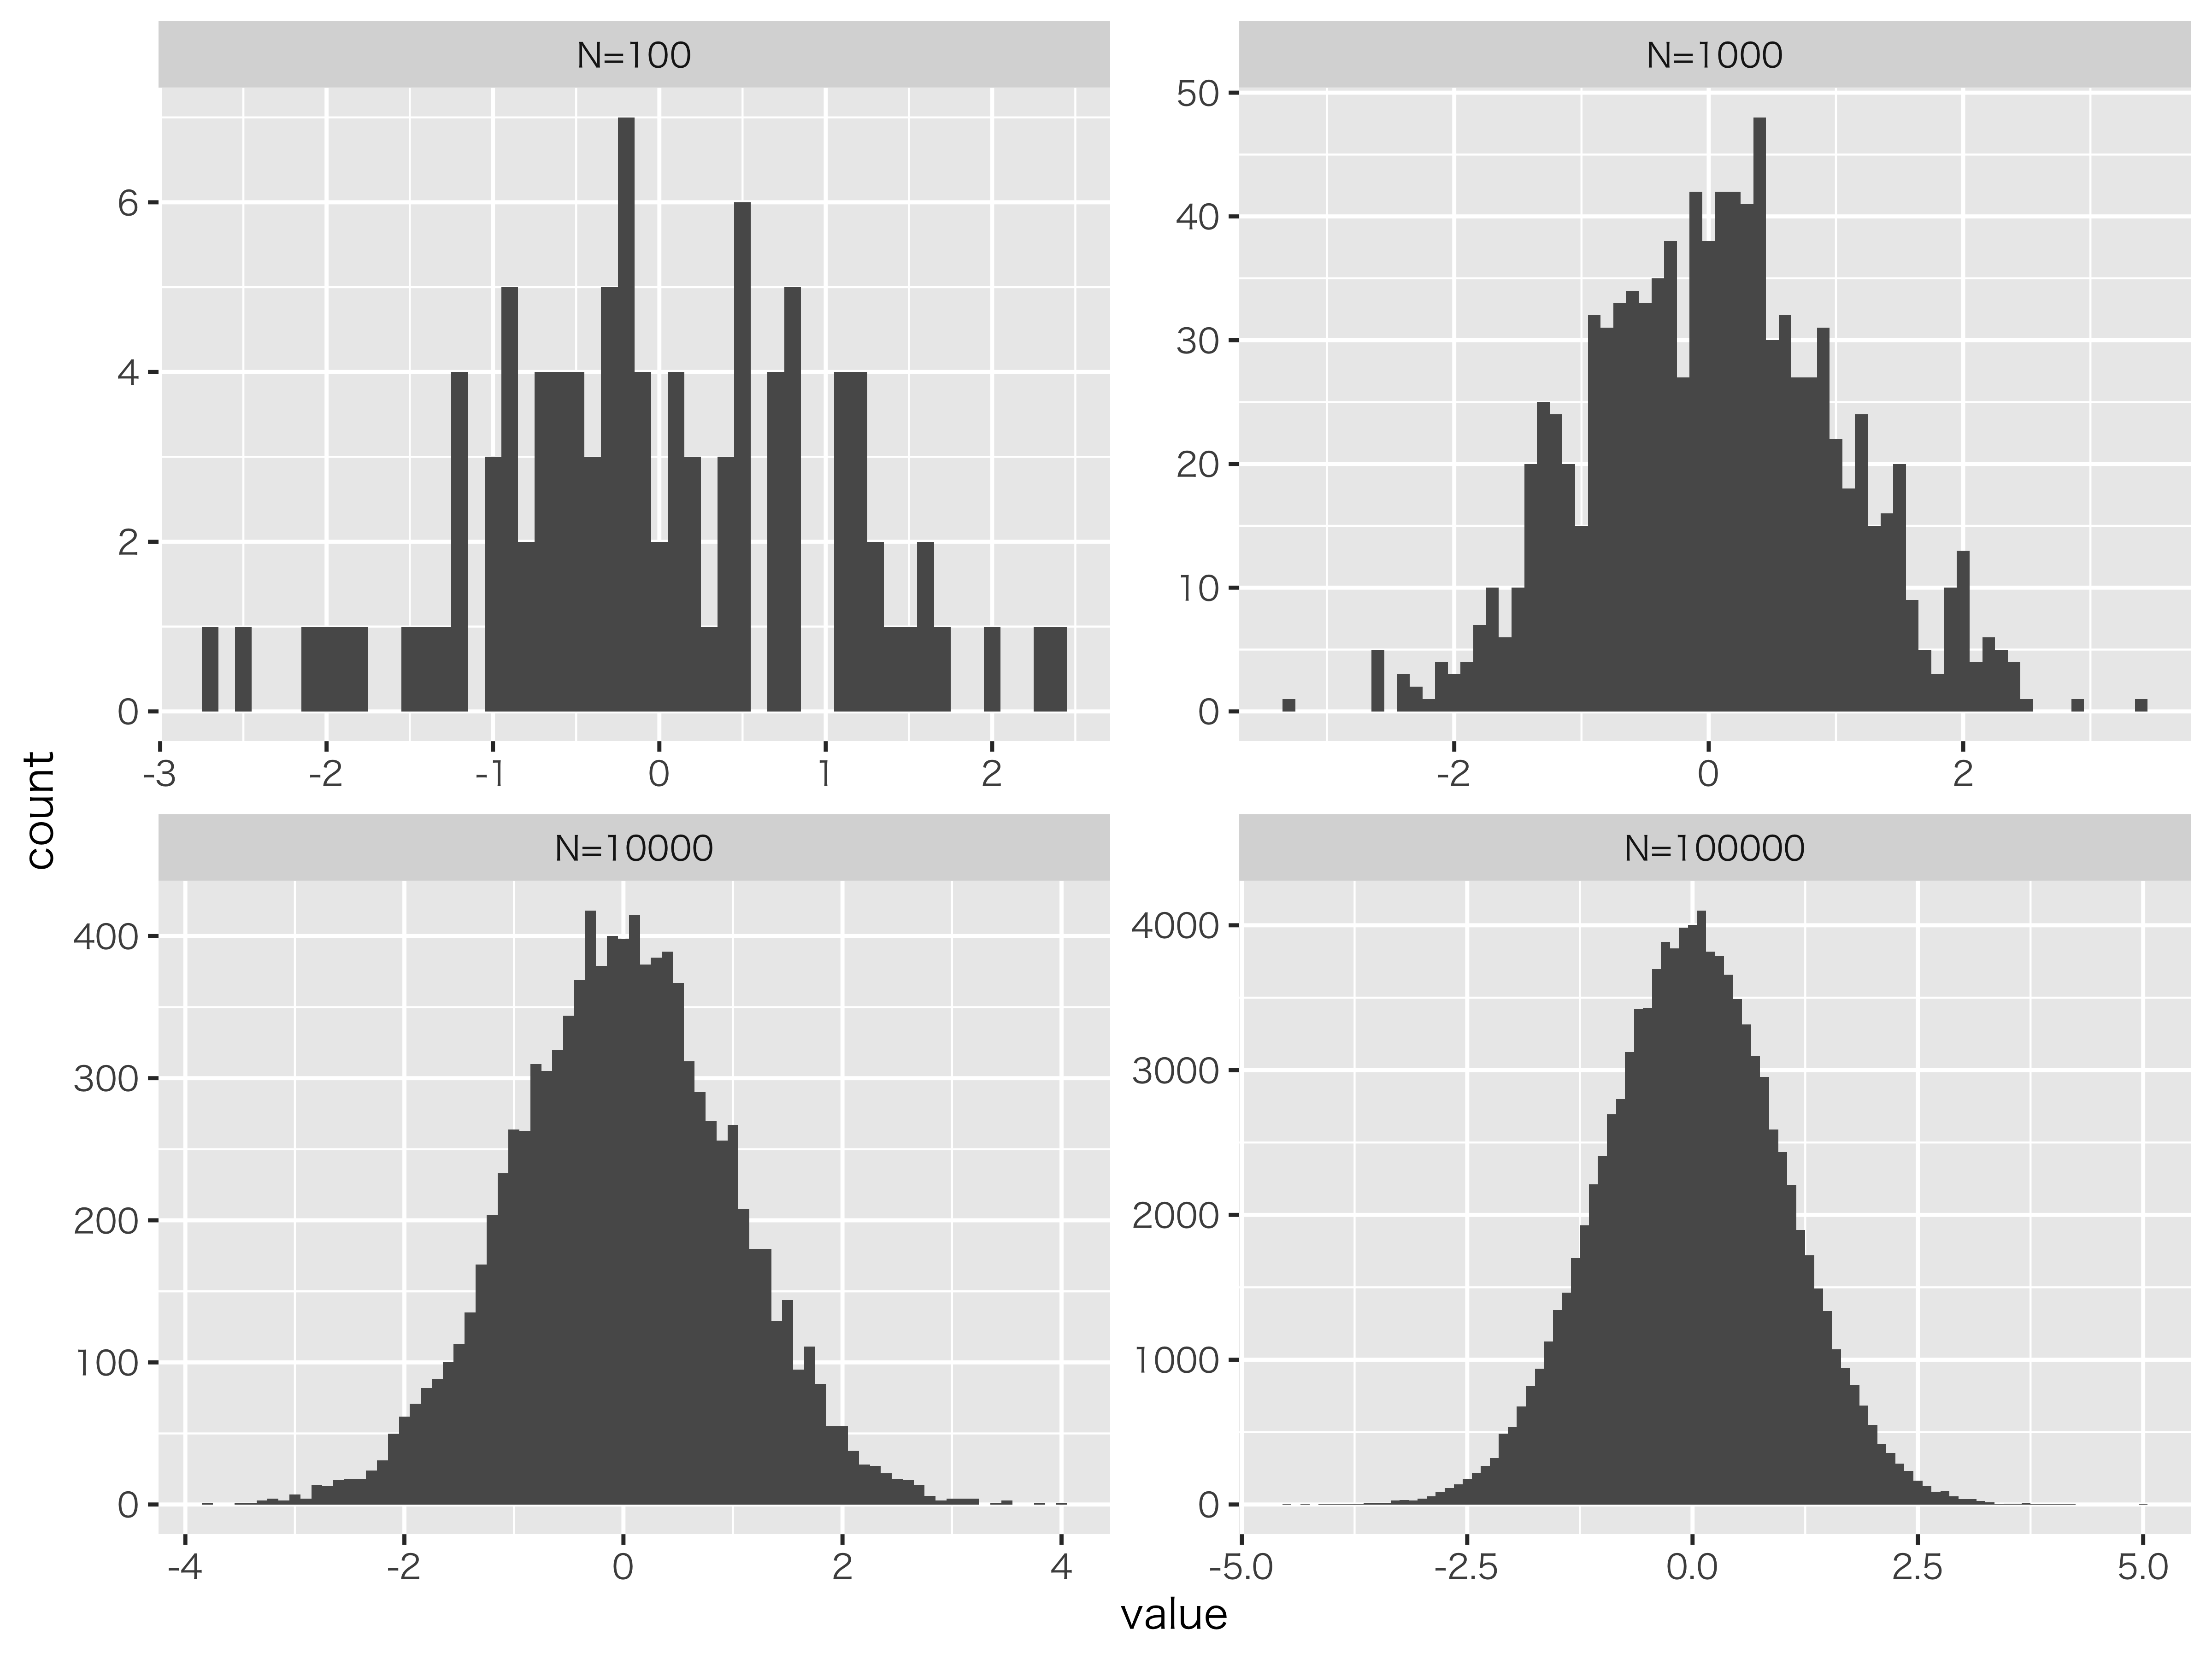
\includegraphics[keepaspectratio,width=8cm]{../images/08_CorrelationCausation/Rplot08_06.png}
    \caption{乱数が増えると正規分布の形に近づく。左上から順に100,1000,10000,100000点の乱数を発生させて描いたヒストグラム}
    \label{fig::08_11}
\end{figure}

このように，発生させる乱数の個数が多くなると，理論的な形(今回は標準正規分布)の近似として十分利用できることになります。
発生させた乱数はそれぞれデータとして扱えますから，このデータの中で例えば0.3より大きく1.0より小さいものの個数を数え，発生させた乱数の数で割ってやる，すなわち相対頻度にすることで確率の計算をできます。
具体例を見てみましょう。

\begin{lstlisting}[language=c++,label={code::08_02},caption={乱数を使った近似}]
    X <- rnorm(n = 100000 , mean = 0 , sd = 1)
    length(X[X>0.3 & X<1.0])
    length(X[X>0.3 & X<1.0])/100000
\end{lstlisting}
\paragraph{コード解説}
\begin{description}
    \item[1行目] 平均0，標準偏差1の正規乱数を10万個発生させ，Xに保存する。
    \item[2行目] \texttt{length}関数はベクトルの長さを返す関数。オブジェクト\texttt{X}のなかでも，条件\verb|X>0.3 & X<1.0|に合致するものだけを抜き出し，その長さを算出。
    \item[3行目] 条件に該当するデータの個数を10万で割ることで相対頻度にする。相対頻度は確率の数字として解釈できる。
\end{description}

\begin{Rscreen}{乱数を使った近似}{out08_02}
\begin{verbatim}
> X <- rnorm(n = 100000 , mean = 0 , sd = 1)
> length(X[X>0.3 & X<1.0])
[1] 22371
> length(X[X>0.3 & X<1.0])/100000
[1] 0.22371
\end{verbatim}
\end{Rscreen}
この方法でも，結果はご覧の通り0.223という他の数字と同じぐらいの値を得ることができました。もちろん乱数ですので，もう一度やると小数点下何桁かのところで違う数字が出てくるかもしれません。その精度をあげたい時は，乱数の発生個数を増やしてやるといいでしょう。例えば10倍にすれば，さらに小数点下1桁ぶんの精度が上がることになります。この方法は，コンピュータの計算能力が高くなったからこそ使えるようになった技で，なんだかかえって面倒な方法のようにも見えますが，実はこの方法が最近になって俄然活用されるようになってきたのです！


\section{まとめにかえて}
話をまとめておきましょう。

正規分布には，大きく分けて2つの意味があります。
ひとつは誤差の分布として，です。特に偶然誤差はどの程度散らばるかということがわかれば，それを見込んで評価できる＝ある程度誤差を飼い慣らすことができる，というのがその利点です。データ＝真値+誤差，という古典的テスト理論モデルは誤差が正規分布すると仮定します。その期待値がゼロになることから，データが十分たくさんあれば真値に辿り着くことができると考えるのでした。

もうひとつ，正規分布を集団全体の傾向を表す分布として理解できます。特に平均（期待値）がどのあたりにあるかに注目し，トレンドを掴むことができるようになります。たとえば平均身長や平均寿命など，社会的にデータを蓄積することでその傾向を考えることができますね。これは個人の特徴＝期待値+個人差，という考え方であり，心理学全域に関わるモデルです。平均的な傾向を探ったり，比較したりすることで議論を進めるためにこの全体的な特徴を利用するのです。

正規分布の第二の意味(集合データの傾向)からは，正規分布の特徴をつかってそのデータの相対的な位置・割合い(ex.何パーセンタイルの辺りにいるか，等)を推測するのに用いることができます。
その際，正規分布の式に平均と分散を入れて計算することもできますが，計算が複雑になるので，データの方を標準化し，標準正規分布と照らし合わせて解釈することが一般的です。
分布を仮定することで，一部のデータから全体を推測する，というのは心理統計の醍醐味の1つでもあるわけです。

正規分布の凄さがわかってもらえましたでしょうか。